\documentclass[sigconf]{acmart}

\usepackage{booktabs}
\usepackage{enumitem}
\usepackage{graphicx}
\graphicspath{{figures/}}
\usepackage{xcolor}
\usepackage{multirow}
\usepackage{csquotes}
\usepackage{siunitx}
\sisetup{group-separator={,}, group-minimum-digits=4}
\usepackage[capitalise,noabbrev]{cleveref}

\AtBeginDocument{%
  \providecommand\BibTeX{{%
    Bib\TeX}}}

\setcopyright{none}
\copyrightyear{2026}
\acmYear{2026}
\acmDOI{}
\acmConference[WebSciEng '26]{Web Science and Engineering}
  {2026}{Delft, The Netherlands}
\acmISBN{}

\begin{document}

\title{From Crowd Knowledge to AI-Assisted Development:\\
A Longitudinal Semantic Analysis of
Stack Overflow After 2020}

\author{Roham Koohestani}
\affiliation{%
  \institution{Delft University of Technology}
  \city{Delft}
  \country{The Netherlands}}
\email{r.koohestani@student.tudelft.nl}

\author{Aditya Patil}
\affiliation{%
  \institution{Delft University of Technology}
  \city{Delft}
  \country{The Netherlands}}
\email{a.c.patil-1@student.tudelft.nl}

\author{Tomasz Sor\'{o}bka}
\affiliation{%
  \institution{Delft University of Technology}
  \city{Delft}
  \country{The Netherlands}}
\email{t.j.sorobka-1@student.tudelft.nl}

% =====================================================================
\begin{abstract}
Stack Overflow has served as the central
knowledge-sharing platform for software developers
for close to two decades.
The public release of ChatGPT in November~2022
triggered a structural shift in how the platform is used.
We analyse \num{24} million questions
from the official Stack Exchange data dump
(\num{60} million posts, \num{189} million rows
across five tables),
covering 75 consecutive months
from January~2020 through March~2026.
Monthly question volume fell by 98.6\,\%,
median response times tripled,
and question body length and code content
each grew by roughly one third;
we find this to be consistent
with an \enquote{AI verification tax}
where developers reserve Stack Overflow
for problems that AI cannot resolve.
Intent classification across nine categories
reveals a tenfold increase in AI-debugging
questions and an 8.1-percentage-point decline
in basic API-usage queries.
All four technology domains
(Legacy Stable, Fast-Moving Web, AI/ML, Other)
lost 69--76\,\% of their mean monthly volume.
Chow structural-break tests confirm
significant breaks at the ChatGPT release
for every tracked metric ($p < 0.012$),
and interrupted time-series regressions
quantify both level and slope changes.
The full pipeline and analysis code are
publicly reproducible.
\end{abstract}

\keywords{Stack Overflow, Developer Communities,
Longitudinal Analysis, Generative AI,
Topic Modelling, Structural Break Analysis}

\maketitle

% =====================================================================
\section{Introduction}
\label{sec:intro}

\subsection{Motivation}

Stack Overflow has served as the public memory
of software engineering since its launch in 2008.
Developers post technical questions,
share solutions,
and document issues that official manuals
fail to cover.
The platform's structured data
(timestamps, voting scores, tags, rich text)
makes it a well-suited subject
for Web Science research.

The release of ChatGPT in
November~2022~\cite{openai2022chatgpt}
disrupted this model.
Developers can now obtain instant answers
from an AI assistant
instead of posting to a public forum.
Programming assistance has moved
from a shared public conversation
to a private one,
which threatens the accumulation
of new public knowledge.
Stack Overflow has not become obsolete,
but the reason people use it has changed.

The 2025 Stack Overflow Developer Survey~\cite{stackoverflow2025survey}
puts numbers on this change:
84\,\% of professional developers
use or plan to use AI tools,
yet 46\,\% distrust AI accuracy.
The most cited frustration (66\,\%)
is \enquote{AI solutions that are almost right,
but not quite},
and 45\,\% report that debugging AI-generated code
consumes excessive time.

\subsection{Problem Statement}

The decline in Stack Overflow activity since late~2022
is well documented.
We argue that the underlying shift is
an \emph{AI verification tax}:
AI handles routine coding queries privately,
so the questions that reach Stack Overflow
are harder, more architectural,
and more frequently about debugging
AI-generated logic.
Stack Overflow itself recognised this change
and expanded support for open-ended,
opinion-based questions in early~2026.
This paper measures that transition
with empirical data.

\subsection{Research Questions}

\begin{description}[leftmargin=*,labelwidth=2.2em]
  \item[RQ1] How have Stack Overflow activity levels,
    answer availability, and response speeds
    changed since 2020?
  \item[RQ2] Did the difficulty and complexity
    of Stack Overflow questions increase after 2022,
    and does this reflect the verification tax?
  \item[RQ3] How did the distribution
    of topics and developer intent shift since 2020?
  \item[RQ4] Which technical domains show
    the strongest changes, and does this
    reveal AI concept drift?
  \item[RQ5] Are the observed shifts
    statistically significant structural breaks,
    and how do level and slope changes decompose
    at the ChatGPT release?
\end{description}

\subsection{Contributions}

\begin{enumerate}[leftmargin=*]
  \item A 75-month longitudinal study
    of \num{24}~million Stack Overflow questions
    with concrete numerical findings
    for five research questions.
  \item A nine-category intent taxonomy
    that extends the Beyer et
    al.\ framework~\cite{beyer2020kind}
    with two AI-era categories.
  \item A per-domain comparison
    across four technology groups
    that documents uniform decline.
  \item Formal structural-break analysis
    (Chow, CUSUM, interrupted time-series regression)
    at the ChatGPT release date.
\end{enumerate}

% =====================================================================
\section{Background and Related Work}
\label{sec:background}

\subsection{Stack Overflow as a Developer
Knowledge Platform}

Stack Overflow launched in 2008 and has since become
the largest question-and-answer site
for software developers.
Questions are tagged by technology,
answers are ranked by community votes,
and questioners mark a single answer as accepted.
This structure has made the platform
a primary data source
for empirical software engineering research.
The Google BigQuery public
dataset~\cite{stackoverflowbigquery2016}
enabled much of this work,
but that snapshot was last refreshed
on 2022-09-25
and cannot be used for AI-era studies.

\subsection{Developer Intent and
Question Taxonomies}

\citet{barua2014developers} applied \textsc{lda}
topic modelling to identify discussion topics
and trends on Stack Overflow.
\citet{allamanis2013and} classified questions
by topic, type, and code structure.
\citet{wang2013empirical} studied
developer interaction patterns.
\citet{beyer2020kind} introduced
a seven-category taxonomy of question types
(\textsc{api} Usage, Discrepancy, Errors,
Review, Conceptual, \textsc{api} Change, Learning)
and evaluated automated classifiers.
We extend the Beyer taxonomy
with two AI-era categories.

\subsection{Developer Behaviour
in the Generative AI Era}

\citet{dasilva2025llms}
examined the reliability and impact of \textsc{llm}s
on Stack Overflow activity
and documented early signs of the decline.
Our study adds a longer observation window
(through March~2026),
formal structural-break tests,
and domain-level decomposition.

% =====================================================================
\section{Data Collection}
\label{sec:data}

\subsection{Choice of Data Source}

We initially planned to query the Stack Overflow
public dataset on Google BigQuery.
That snapshot was last refreshed on 2022-09-25,
two months before ChatGPT's release,
and is therefore useless for our purposes.
A community-mirrored Stack Exchange dump
on the Internet Archive proved incomplete,
ending in early~2024.
We therefore use the \textbf{official
Stack Exchange data dump},
downloaded from the Stack Overflow
Data Dump settings page.
Our copy covers all posts
through \textbf{2026-03-31}.
The archive's \textsc{sha}-256 fingerprint
is recorded in
\texttt{results/tables/manifest.yaml}.

\subsection{Tables Used}

The official dump contains eight tables.
We extract five:
\textbf{Posts} (questions and answers,
distinguished by \texttt{PostTypeId}),
\textbf{Users}, \textbf{Comments},
\textbf{PostLinks}, and \textbf{Tags}.
The remaining three (Badges,
PostHistory, Votes) are irrelevant
to our research questions.

\subsection{Local Ingestion Pipeline}

Each table is extracted from a single
\texttt{.7z} archive.
We stream \textsc{xml} through
\texttt{lxml.iterparse}
(constant-memory parsing)
and write monthly-partitioned Parquet
via \texttt{pyarrow.ParquetWriter}.
The partition key is
\texttt{year\_month=YYYY-MM},
derived from each row's \texttt{CreationDate}.
The full pipeline finishes
in approximately three hours
on a 2024 MacBook Air;
the 60-million-row Posts table
dominates the runtime.
A private Hugging Face repository
hosts the materialised Parquet
for co-author access.

\subsection{Data Validation}

\Cref{tab:data-summary} shows
the ingested dataset.
The analysis window covers
\textbf{75 consecutive months}
from January~2020 through March~2026
with \textbf{zero gaps}.
Question volume dropped
from \num{146664} in January~2020
to \num{2033} in March~2026,
a 98.6\,\% decline.

\begin{table}[t]
  \caption{Dataset summary after ingestion.}
  \label{tab:data-summary}
  \centering
  \begin{tabular}{l
    S[table-format=11.0]
    S[table-format=3.0]
    ll}
    \toprule
    Table & {Rows} & {Parts.}
      & {First Date} & {Last Date} \\
    \midrule
    Posts     & 60349494 & 213
      & 2008-07-31 & 2026-03-31 \\
    Users     & 31031671 & 213
      & 2008-07-31 & 2026-03-31 \\
    Comments  & 91268612 & 212
      & 2008-08-01 & 2026-03-31 \\
    PostLinks &  6523169 & 192
      & 2010-04-26 & 2026-03-31 \\
    Tags      &    65941 &   1
      & {---} & {---} \\
    \midrule
    \textbf{Total}
      & \textbf{189238887} & & & \\
    \bottomrule
  \end{tabular}
\end{table}

\subsection{Sampling Methodology}

Metrics computed via \textsc{sql} aggregation
(\textsc{rq}1, \textsc{rq}4)
operate on the \emph{full population}
of six million questions
in the analysis window.
Analyses that require per-post text processing
(\textsc{rq}2, \textsc{rq}3)
use a power-analysis-driven stratified sample.
Per month, the required sample size
is the larger of two values:
(1)~a power-based criterion
(Cohen's $h = 0.2$,
$\alpha = 0.05$, power $= 0.95$) and
(2)~a margin-of-error criterion
targeting $\pm 2$~percentage points
with Bonferroni correction
for $k$~simultaneous comparisons.
Both apply a finite-population correction.
The resulting cap is approximately
\num{4700}~questions per month
for intent classification ($k=9$)
and \num{4250} for lexical features ($k=6$),
yielding \num{312000}--\num{343000} sampled posts
(4.7--5.2\,\% of the population).
Sampling is deterministic via hash-ordered
row numbers and thus reproducible.

% =====================================================================
\section{Data Analysis}
\label{sec:analysis}

\subsection{Activity Trends and
Interaction Speeds (RQ1)}
\label{sec:rq1}

We track seven monthly time series
across 75~months,
split at the ChatGPT release
on 2022-11-30
(35~pre-release months, 40~post).
\Cref{fig:activity,fig:quality,%
fig:response-time,fig:engagement}
show the results.

\begin{figure}[t]
  \centering
  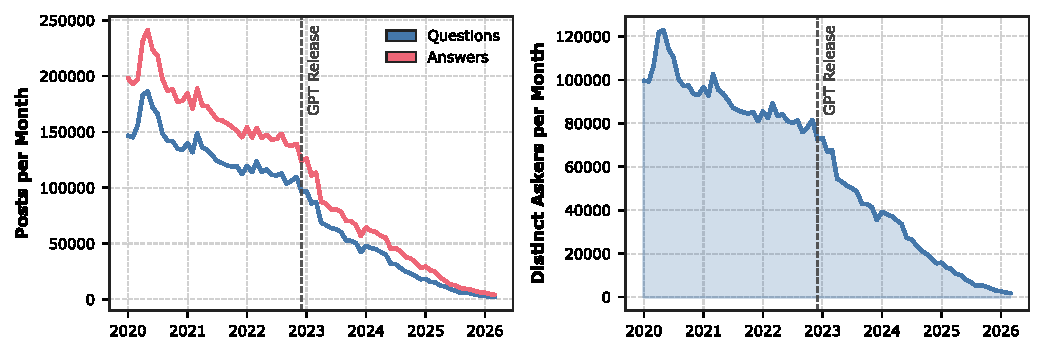
\includegraphics[width=\columnwidth]{one_activity}
  \caption{Monthly question and answer volume
    (left) and distinct askers (right).
    The dashed line marks the ChatGPT release.}
  \label{fig:activity}
\end{figure}

\paragraph{Volume.}
Question and answer volume collapsed.
Median monthly questions fell
from \num{129018} pre-ChatGPT
to \num{29682} post ($-77\,\%$).
The endpoint contrast is sharper:
\num{146664} questions in January~2020
versus \num{2033} in March~2026 ($-98.6\,\%$).
Answers tracked questions in lockstep:
median \num{166903} to \num{43968}
per month ($-74\,\%$).

\paragraph{Active askers.}
Distinct non-anonymous askers per month
fell from a pre-ChatGPT median
of \num{90649} to \num{25130} ($-72\,\%$).
The questions-per-asker ratio decreased
from 1.42 to 1.18 ($-17\,\%$).
The platform thinned because
\emph{fewer people came at all};
the surviving users did not shed
most of their questions.

\begin{figure}[t]
  \centering
  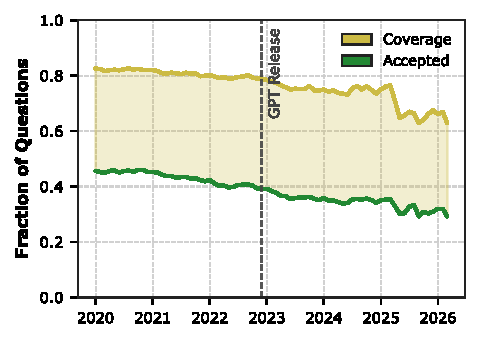
\includegraphics[width=\columnwidth]{one_quality}
  \caption{Monthly accepted-answer rate
    and answer coverage rate.}
  \label{fig:quality}
\end{figure}

\paragraph{Quality.}
The accepted-answer rate fell
from 43.2\,\% pre to 35.0\,\% post
($-8$~pp).
Answer coverage dropped
from 80.9\,\% to 73.9\,\% ($-7$~pp).
The gap between coverage and acceptance
stayed flat
(37.6\,\% pre vs.\ 38.8\,\% post),
which contradicts the hypothesis
that the community keeps answering
while askers stop returning to accept.

\begin{figure}[t]
  \centering
  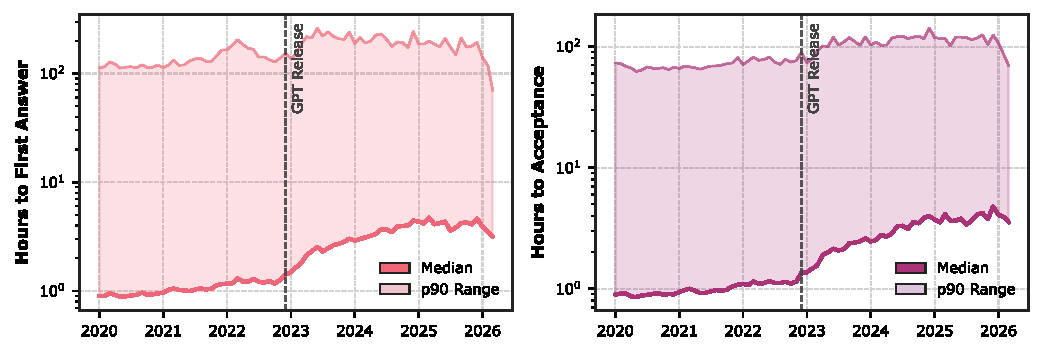
\includegraphics[width=\columnwidth]{one_response_time}
  \caption{Median hours to first answer (left)
    and to acceptance (right),
    with p90 bands. Log scale.}
  \label{fig:response-time}
\end{figure}

\paragraph{Response times.}
Median time-to-first-answer tripled:
\qty{1.0}{h} pre to \qty{3.5}{h} post
($\times 3.4$).
Time-to-acceptance followed:
\qty{1.0}{h} to \qty{2.8}{h}
($\times 2.9$).
The median rose faster than the p90 tail,
so the slowdown is platform-wide
and not concentrated in hard questions.

\begin{figure}[t]
  \centering
  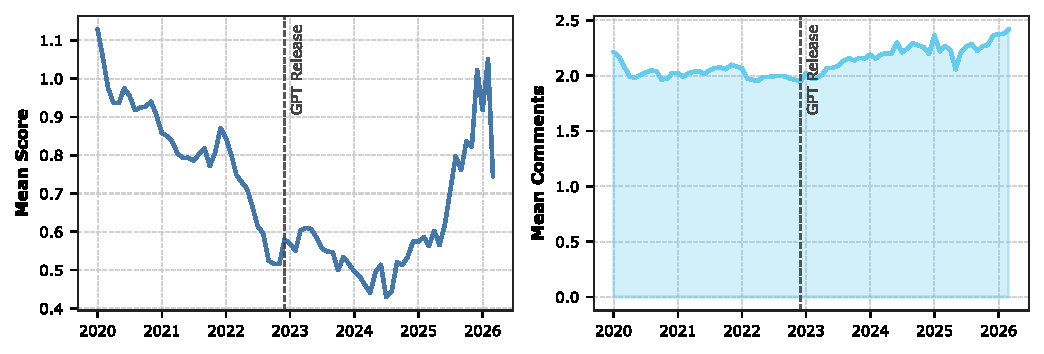
\includegraphics[width=\columnwidth]{one_engagement}
  \caption{Mean question score (left)
    and mean comments per question (right).}
  \label{fig:engagement}
\end{figure}

\paragraph{Engagement.}
Mean question score fell
from 0.82 to 0.61 ($-25\,\%$).
Mean comment count rose
from 2.03 to 2.20 ($+8\,\%$).
The surviving questions receive
more discussion but fewer upvotes.

% -----------------------------------------------------------------
\subsection{Question Complexity
and Difficulty (RQ2)}
\label{sec:rq2}

We compute six lexical features per question:
title length,
body prose length
(excluding \texttt{<pre>} regions),
total code-block length,
code-block count, link count,
and tag count.
Features are extracted on a stratified
monthly sample
(cap \num{4252} per month)
and aggregated to monthly median and p90.
\Cref{fig:complexity-trends} plots
the time series;
\Cref{fig:complexity-change} shows
pre/post percentage changes.

\begin{figure}[t]
  \centering
  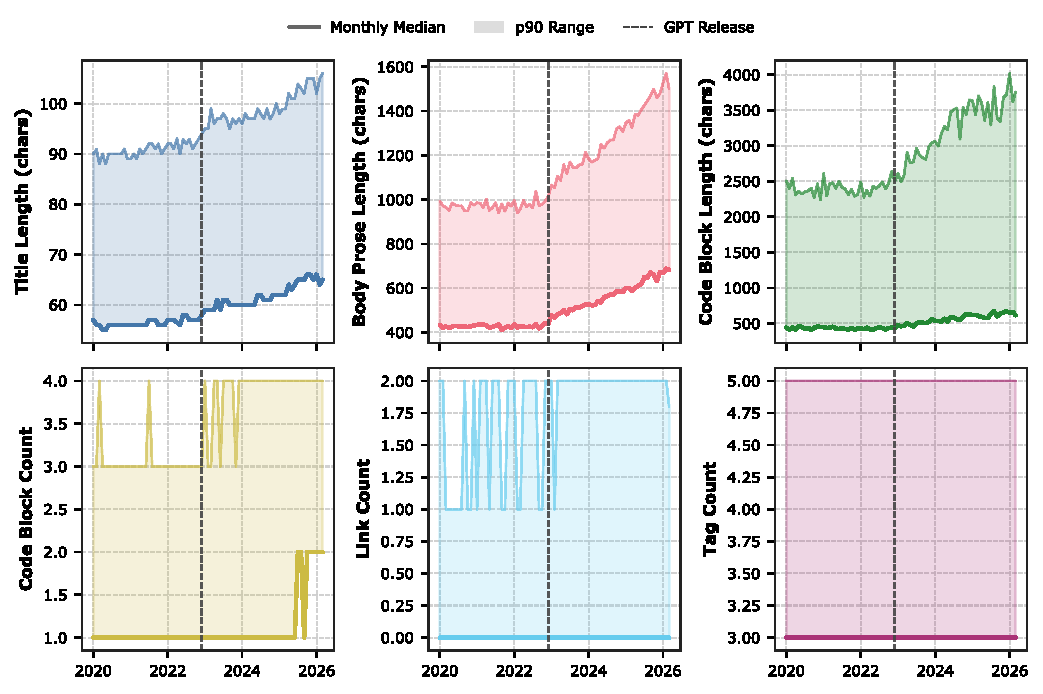
\includegraphics[width=\columnwidth]{two_complexity_trends}
  \caption{Six lexical features over time:
    monthly median (line) and p90 band.
    The dashed line marks the ChatGPT release.}
  \label{fig:complexity-trends}
\end{figure}

\begin{figure}[t]
  \centering
  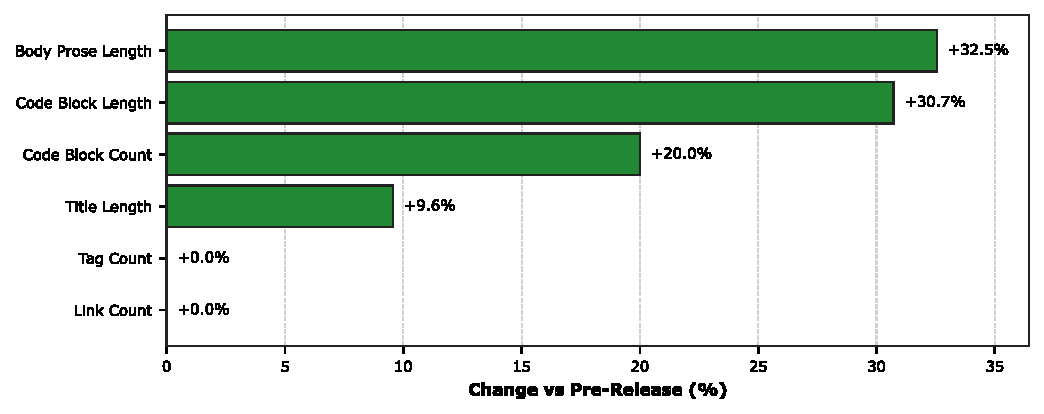
\includegraphics[width=\columnwidth]{two_complexity_change}
  \caption{Percentage change in mean-of-monthly-medians,
    pre vs.\ post ChatGPT release.}
  \label{fig:complexity-change}
\end{figure}

\paragraph{Body prose length}
showed the largest change.
The monthly median rose from 428~characters pre
to 567 post ($+32.3\,\%$);
the p90 rose from 972 to \num{1273}
($+30.9\,\%$).
\paragraph{Code-block total length}
increased from 432 to 565~characters
($+30.9\,\%$),
mirroring prose growth.
Post-release questions contain
more text \emph{and} more code;
one did not substitute for the other.
\paragraph{Code-block count}
rose at the median
from 1.00 to 1.18 ($+17.5\,\%$).
By mid-2025 the typical question
contains two separate code blocks.
\paragraph{Title length}
grew from 56.5 to 61.8~characters
($+9.3\,\%$).
\paragraph{Link count}
held at zero at the median;
the p90 rose from 1.57 to 1.98
($+25.7\,\%$).
\paragraph{Tag count}
was flat (median~3, p90~5)
because the \textsc{ui} enforces
a hard five-tag cap.

Every content-size feature increased,
while platform-constrained features
held flat.
Median and p90 grew within
three percentage points of each other
for every length feature,
so the shift is population-wide.
The pattern fits the verification-tax
mechanism:
questions that AI resolves
no longer reach Stack Overflow,
and the residual is heavier
in every free-to-vary content dimension.

% -----------------------------------------------------------------
\subsection{Topic and Intent Distribution (RQ3)}
\label{sec:rq3}

Each sampled question is classified
into one of nine intent categories
by regex-based pattern matching
on the title and parsed body prose.
The taxonomy extends the Beyer et al.\
seven-category framework~\cite{beyer2020kind}
with two AI-era additions:
\emph{Machine-Authored Discrepancy}
(debugging AI-generated code)
and \emph{Architectural Consensus}
(seeking design validation).
The sample comprises
\num{4686}~questions per month
(\num{342945}~total);
patterns are evaluated
in specificity order, most specific first.

\begin{figure}[t]
  \centering
  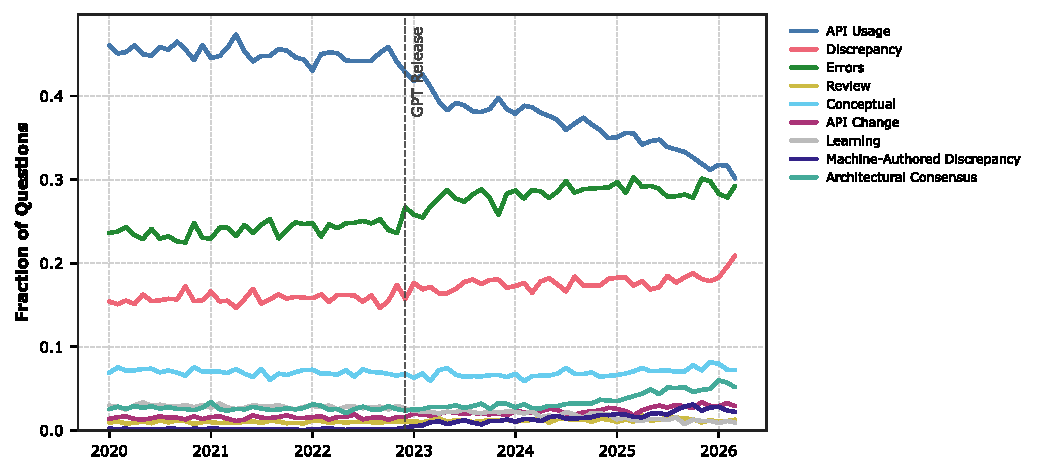
\includegraphics[width=\columnwidth]{three_intent_trends}
  \caption{Monthly fraction of questions
    per intent category.}
  \label{fig:intent-trends}
\end{figure}

\begin{figure}[t]
  \centering
  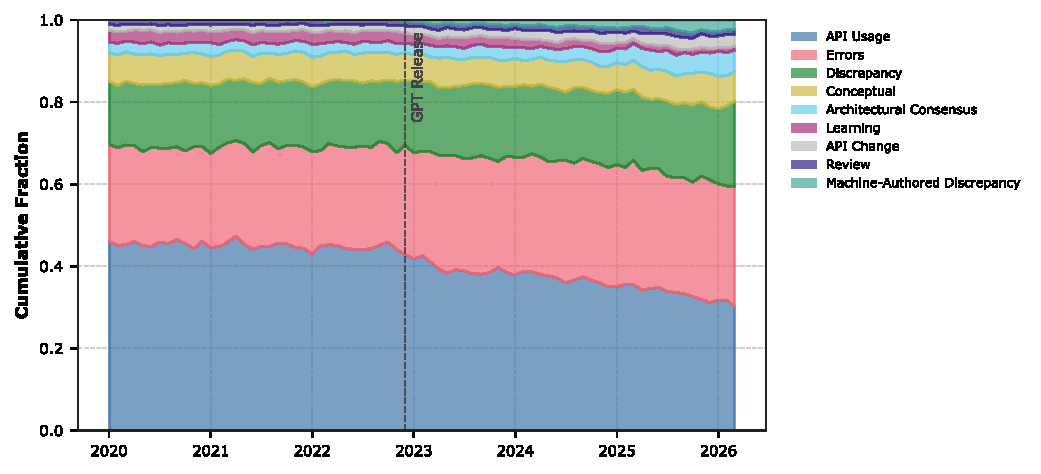
\includegraphics[width=\columnwidth]{three_intent_stacked}
  \caption{Stacked area chart
    of cumulative intent fraction.}
  \label{fig:intent-stacked}
\end{figure}

\Cref{fig:intent-trends} plots the nine
category fractions over time,
and \Cref{fig:intent-stacked} gives
a stacked-area view of the same data.
\Cref{tab:intent-prepost} quantifies
the pre/post shift.

\begin{table}[t]
  \caption{Intent category fractions
    pre and post ChatGPT release.}
  \label{tab:intent-prepost}
  \centering
  \small
  \begin{tabular}{l
      S[table-format=2.1]
      S[table-format=2.1]
      S[table-format=+1.1,
        explicit-sign]}
    \toprule
    Intent
      & {Pre (\%)} & {Post (\%)}
      & {$\Delta$ (pp)} \\
    \midrule
    API Usage        & 45.1 & 37.0 & -8.1 \\
    Errors           & 24.0 & 28.2 & +4.2 \\
    Discrepancy      & 15.7 & 17.6 & +1.9 \\
    Conceptual       &  7.0 &  6.8 & -0.2 \\
    Arch.\ Consensus &  2.7 &  3.5 & +0.9 \\
    Learning         &  2.8 &  1.8 & -1.0 \\
    API Change       &  1.5 &  2.3 & +0.8 \\
    {Mach.-Auth.\ Disc.}
                     & 0.15 &  1.5 & +1.4 \\
    Review           &  1.0 &  1.2 & +0.2 \\
    \bottomrule
  \end{tabular}
\end{table}

\paragraph{Decline in API Usage.}
\textsc{api} Usage,
the \enquote{how do I use X} category,
fell from 45.1\,\% to 37.0\,\% ($-8.1$~pp).
AI assistants handle these queries well,
and the decline is consistent
with displacement to private tools.

\paragraph{Rise in error diagnosis.}
Errors rose from 24.0\,\% to 28.2\,\% ($+4.2$~pp),
and Discrepancy (unexpected behaviour)
rose from 15.7\,\% to 17.6\,\% ($+1.9$~pp).
Troubleshooting categories now account
for 45.8\,\% of post-release questions,
up from 39.7\,\%.

\paragraph{Machine-Authored Discrepancy.}
This AI-era category grew tenfold,
from 0.15\,\% pre to 1.50\,\% post.
The absolute share remains small,
but \Cref{fig:ai-categories} shows
accelerating growth from 2023 onward
as AI-generated code
becomes more prevalent.

\begin{figure}[t]
  \centering
  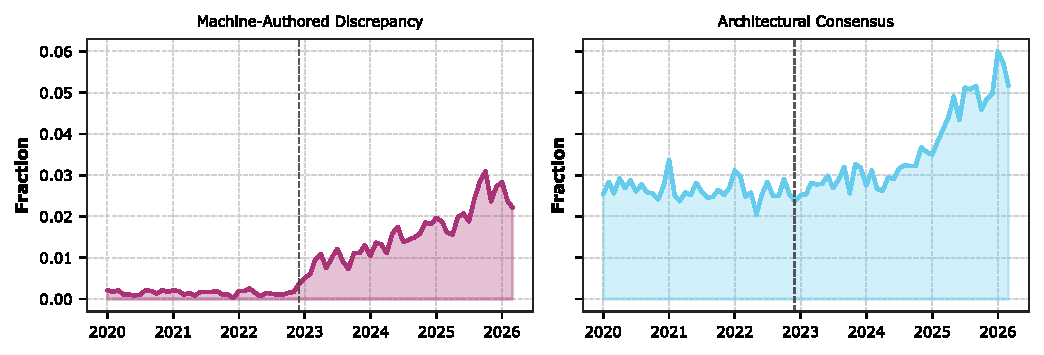
\includegraphics[width=\columnwidth]{three_ai_categories}
  \caption{The two AI-era intent categories:
    Machine-Authored Discrepancy (left)
    and Architectural Consensus (right).}
  \label{fig:ai-categories}
\end{figure}

\begin{figure}[t]
  \centering
  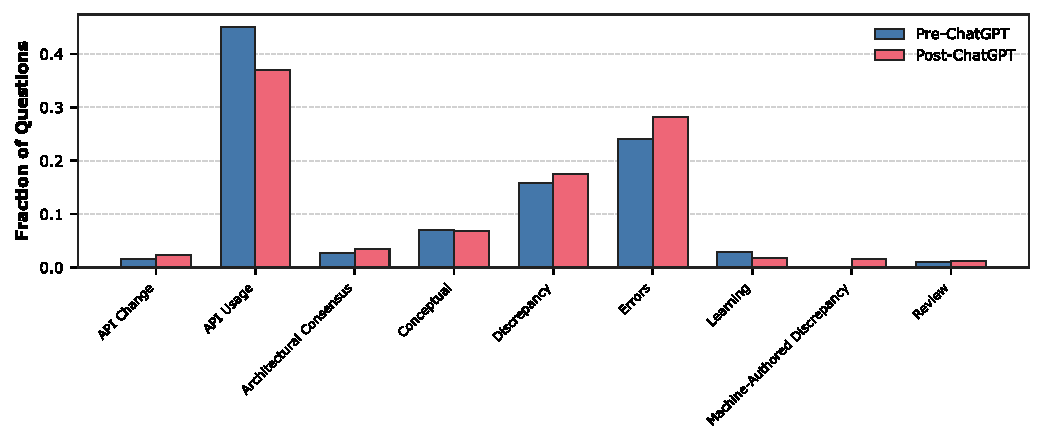
\includegraphics[width=\columnwidth]{three_intent_prepost}
  \caption{Pre vs.\ post ChatGPT
    intent fractions (grouped bars).}
  \label{fig:intent-prepost}
\end{figure}

\paragraph{Architectural Consensus}
grew from 2.7\,\% to 3.5\,\% ($+0.9$~pp).
Developers seek human judgement
on design decisions that AI tools
cannot resolve authoritatively.

\paragraph{Decline in Learning.}
Learning-oriented questions fell
from 2.8\,\% to 1.8\,\% ($-1.0$~pp).
Introductory material is
now obtained from AI instead.

% -----------------------------------------------------------------
\subsection{Tag-Group and
Domain Comparison (RQ4)}
\label{sec:rq4}

We partition questions into four domains
based on tag membership to test
whether the ChatGPT-era shift
is uniform or exhibits concept drift:
\emph{Legacy Stable}
(C++, C\#, Java, \textsc{sql}, etc.),
\emph{Fast-Moving Web}
(JavaScript, React, Angular, Node.js, etc.),
\emph{AI/ML}
(Python, TensorFlow, PyTorch, etc.),
and \emph{Other}.
All domain metrics use the full population.

\begin{figure}[t]
  \centering
  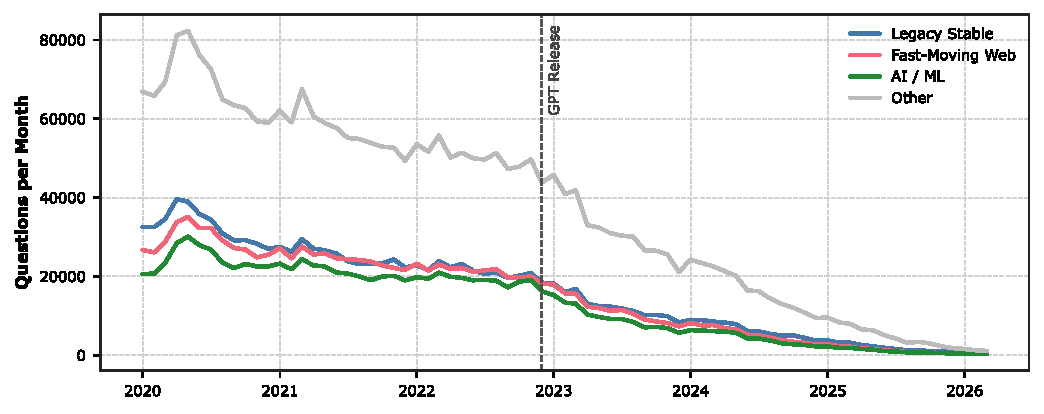
\includegraphics[width=\columnwidth]{four_domain_volume}
  \caption{Monthly question volume
    by technology domain.}
  \label{fig:domain-volume}
\end{figure}

\begin{figure}[t]
  \centering
  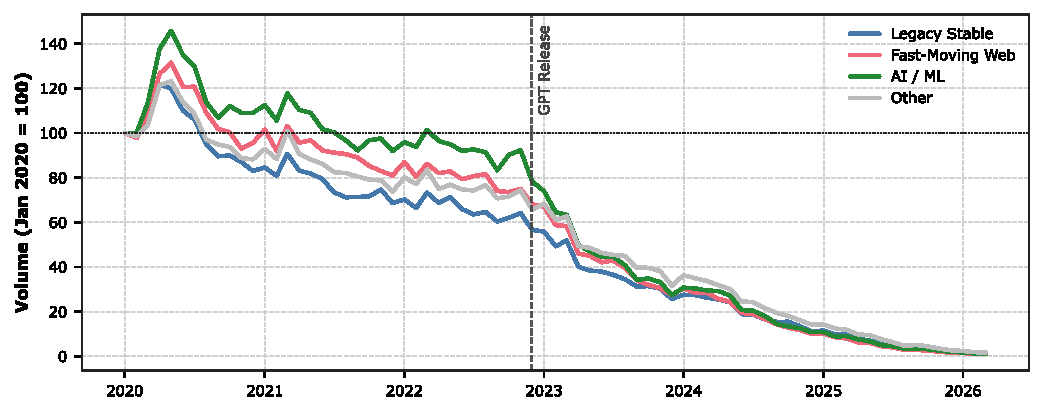
\includegraphics[width=\columnwidth]{four_domain_volume_normalized}
  \caption{Volume indexed
    to January~2020 = 100 per domain.}
  \label{fig:domain-normalized}
\end{figure}

\paragraph{Volume.}
\Cref{fig:domain-volume} shows absolute volume;
\Cref{fig:domain-normalized} normalises
to January~2020.
\Cref{tab:domain-change} reports the decline.
All four domains lost 69--76\,\%
of their mean monthly volume.
AI/ML ($-75.5\,\%$) and Fast-Moving Web
($-75.0\,\%$) fell slightly more
than Legacy Stable ($-73.4\,\%$)
and Other ($-69.2\,\%$),
but the differences are small.
The concept-drift hypothesis,
which predicts that rapidly evolving frameworks
would suffer disproportionately,
finds only weak support.

\begin{table}[t]
  \caption{Mean monthly volume change
    by domain, pre vs.\ post.}
  \label{tab:domain-change}
  \centering
  \begin{tabular}{l
    S[table-format=5.0]
    S[table-format=5.0]
    S[table-format=-2.1]}
    \toprule
    Domain
      & {Pre mean} & {Post mean}
      & {Change (\%)} \\
    \midrule
    AI / ML         & 21722 &  5326 & -75.5 \\
    Fast-Moving Web & 25229 &  6316 & -75.0 \\
    Legacy Stable   & 26815 &  7144 & -73.4 \\
    Other           & 59298 & 18235 & -69.2 \\
    \bottomrule
  \end{tabular}
\end{table}

\begin{figure}[t]
  \centering
  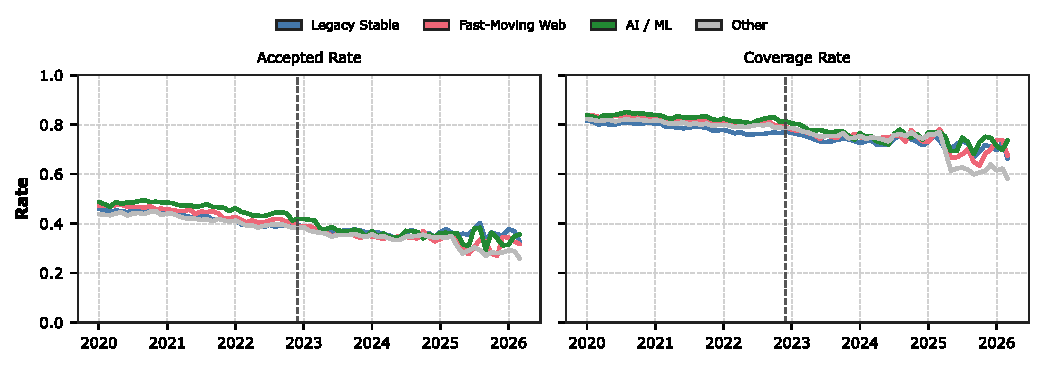
\includegraphics[width=\columnwidth]{four_domain_quality}
  \caption{Accepted rate (left)
    and coverage rate (right) by domain.}
  \label{fig:domain-quality}
\end{figure}

\paragraph{Quality.}
\Cref{fig:domain-quality} shows accepted rate
and coverage rate by domain.
AI/ML had the largest accepted-rate drop
(46.8\,\% to 37.9\,\%, $-8.9$~pp);
Fast-Moving Web dropped
from 44.6\,\% to 36.0\,\% ($-8.6$~pp);
Legacy Stable fell
from 43.0\,\% to 37.0\,\% ($-6.0$~pp).
Coverage rates followed the same pattern.

\begin{figure}[t]
  \centering
  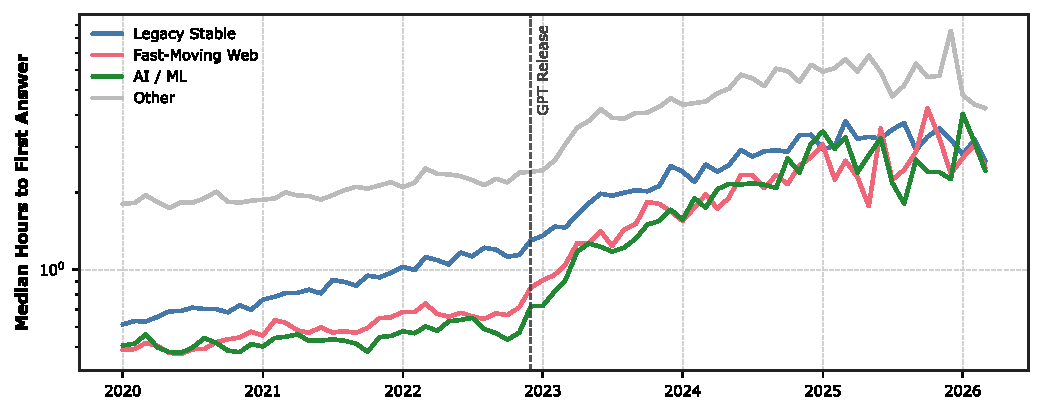
\includegraphics[width=\columnwidth]{four_domain_response_time}
  \caption{Median hours to first answer
    by domain (log scale).}
  \label{fig:domain-response}
\end{figure}

\paragraph{Response times.}
\Cref{fig:domain-response} confirms that
every domain experienced rising
time-to-first-answer.
No domain escaped the slowdown.

\begin{figure}[t]
  \centering
  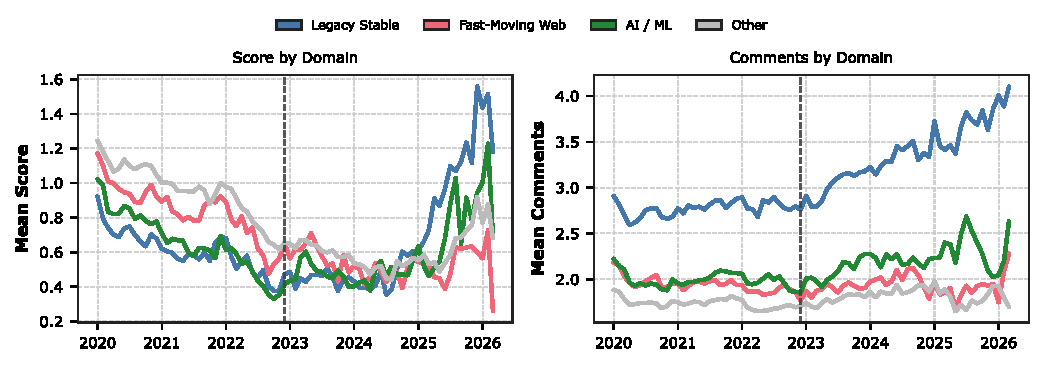
\includegraphics[width=\columnwidth]{four_domain_engagement}
  \caption{Mean score (left)
    and mean comments (right) by domain.}
  \label{fig:domain-engagement}
\end{figure}

\paragraph{Engagement.}
\Cref{fig:domain-engagement} shows
mean score and comments by domain.
Legacy Stable carried the highest
comment counts:
2.77 pre, 3.13 post ($+13\,\%$).
Established-technology questions
attract more back-and-forth.

\begin{figure}[t]
  \centering
  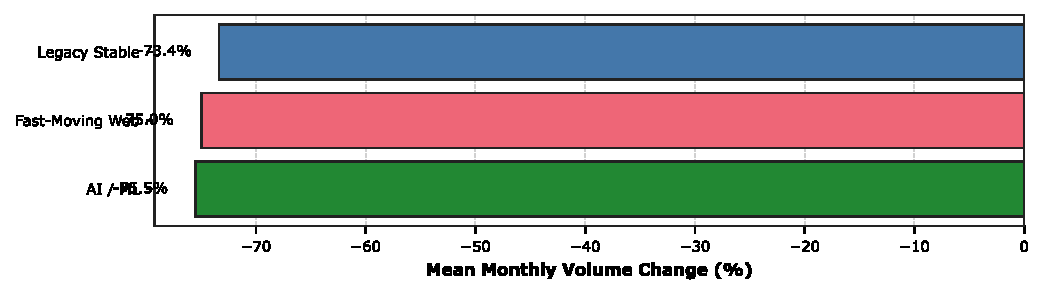
\includegraphics[width=\columnwidth]{four_domain_volume_change}
  \caption{Mean monthly volume change (\%)
    by domain.}
  \label{fig:domain-volume-change}
\end{figure}

% -----------------------------------------------------------------
\subsection{Temporal Statistics (RQ5)}
\label{sec:rq5}

We apply three formal statistical tests
to each of the nine key time series,
with the ChatGPT release (December~2022)
as the hypothesised breakpoint.

\subsubsection{Chow Structural-Break Test}

The Chow test fits a segmented linear regression
(intercept, trend, post-break indicator,
and interaction term)
and compares its residual sum of squares
against a restricted model with no break.
\Cref{tab:chow} shows that
\textbf{all nine metrics}
exhibit a significant structural break
at $\alpha = 0.05$.
The strongest signals come from
Time to Acceptance ($F = 80.46$, $p < 10^{-6}$),
Mean Score ($F = 65.86$),
and Mean Comments ($F = 37.76$).
The weakest, Accepted Rate
($F = 4.80$, $p = 0.011$),
is still significant.

\begin{table}[t]
  \caption{Chow structural-break test results
    at December~2022.}
  \label{tab:chow}
  \centering
  \small
  \begin{tabular}{l
    S[table-format=2.2]
    l}
    \toprule
    Metric & {$F$-stat.} & $p$-value \\
    \midrule
    Time to Accept.\ (med)
      & 80.46 & $< 10^{-6}$ \\
    Mean Score
      & 65.86 & $< 10^{-6}$ \\
    Mean Comments
      & 37.76 & $< 10^{-6}$ \\
    Time to 1st Ans.\ (med)
      & 32.28 & $< 10^{-6}$ \\
    Active Askers
      & 30.27 & $< 10^{-6}$ \\
    Answer Coverage
      & 14.85 & $4 \times 10^{-6}$ \\
    Question Volume
      & 12.92 & $1.6 \times 10^{-5}$ \\
    Answer Volume
      & 11.89 & $3.5 \times 10^{-5}$ \\
    Accepted Rate
      &  4.80 & $0.011$ \\
    \bottomrule
  \end{tabular}
\end{table}

\begin{figure}[t]
  \centering
  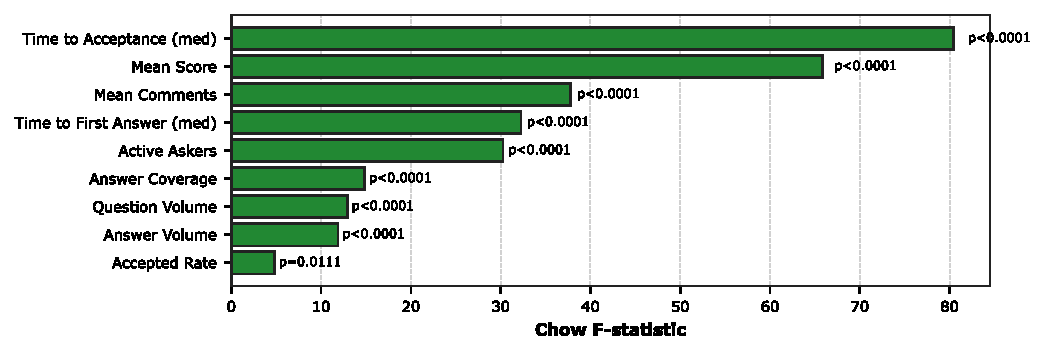
\includegraphics[width=\columnwidth]{five_chow_summary}
  \caption{Chow $F$-statistics per metric.
    Green bars: $p < 0.05$.}
  \label{fig:chow}
\end{figure}

\subsubsection{CUSUM Test}

The \textsc{cusum} test accumulates
\textsc{ols} residuals
under a null hypothesis of linear trend
and compares the maximum cumulative deviation
against the 5\,\% critical boundary.
All nine metrics exceed the critical value
(8.21), confirming pervasive
structural instability.
Volume metrics peak in March~2023,
four months after the release.
Response-time metrics peak later
(October~2023 for first answer).
The lag points to a delayed cascade
from volume collapse
to answering-pipeline deterioration.

\begin{figure}[t]
  \centering
  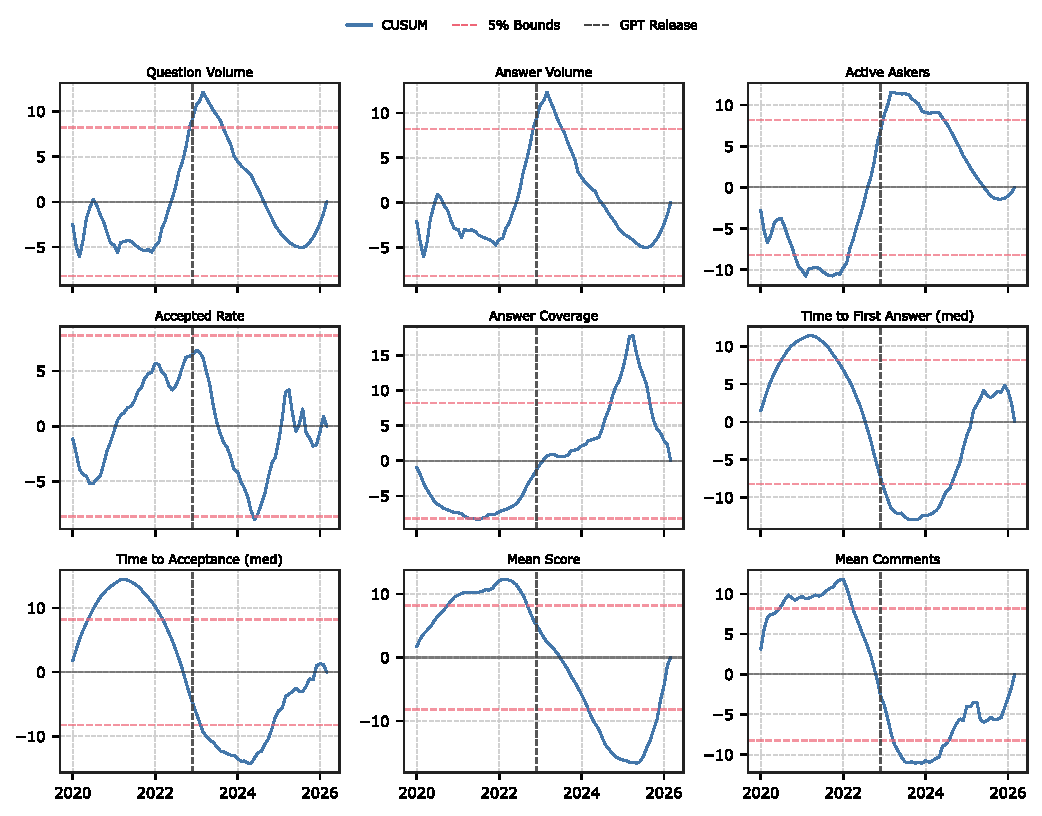
\includegraphics[width=\columnwidth]{five_cusum_paths}
  \caption{\textsc{cusum} paths per metric
    with 5\,\% critical bounds (dashed).}
  \label{fig:cusum}
\end{figure}

\subsubsection{Interrupted Time-Series Regression}

We fit the \textsc{its} model
$y_t = \beta_0 + \beta_1 t
  + \beta_2 D_t + \beta_3 T_t^{\text{post}}
  + \varepsilon_t$,
where $D_t$ is a post-break indicator
and $T_t^{\text{post}}$ counts months
since the break.
\Cref{tab:its} reports the level change
($\beta_2$) and slope change ($\beta_3$).

\begin{table}[t]
  \caption{\textsc{its} regression:
    level and slope change at December~2022.}
  \label{tab:its}
  \centering
  \small
  \begin{tabular}{lrlrl}
    \toprule
    Metric
      & {$\beta_2$ (level)} & $p$
      & {$\beta_3$ (slope)} & $p$ \\
    \midrule
    Question Vol.
      & $-$\num{18960} & $<10^{-4}$
      & $-502$ & $0.010$ \\
    Answer Vol.
      & $-$\num{22234} & $<10^{-4}$
      & $-454$ & $0.044$ \\
    Active Askers
      & $-$\num{10722} & $<10^{-4}$
      & $-808$ & $<10^{-6}$ \\
    Accepted Rate
      & $-0.014$ & $0.004$
      & $+0.0001$ & $0.641$ \\
    Ans.\ Coverage
      & $+0.003$ & $0.713$
      & $-0.002$ & $<10^{-6}$ \\
    1st Answer (s)
      & $+$\num{2743} & $<10^{-4}$
      & $+194$ & $<10^{-6}$ \\
    Acceptance (s)
      & $+$\num{1748} & $<10^{-4}$
      & $+226$ & $<10^{-6}$ \\
    Mean Score
      & $-0.130$ & $0.004$
      & $+0.021$ & $<10^{-6}$ \\
    Mean Comments
      & $+0.047$ & $0.087$
      & $+0.011$ & $<10^{-6}$ \\
    \bottomrule
  \end{tabular}
\end{table}

\begin{figure}[t]
  \centering
  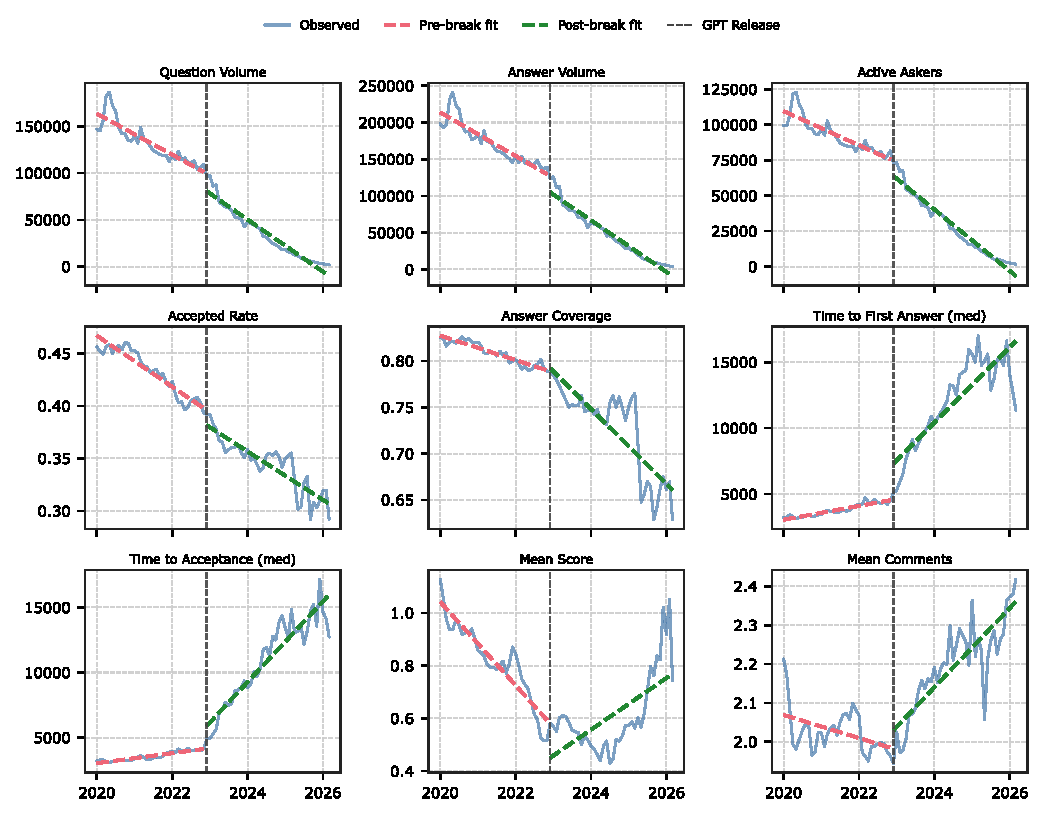
\includegraphics[width=\columnwidth]{five_its_fits}
  \caption{\textsc{its} fits per metric.
    Solid: observed. Dashed: fitted segments.}
  \label{fig:its-fits}
\end{figure}

\begin{figure}[t]
  \centering
  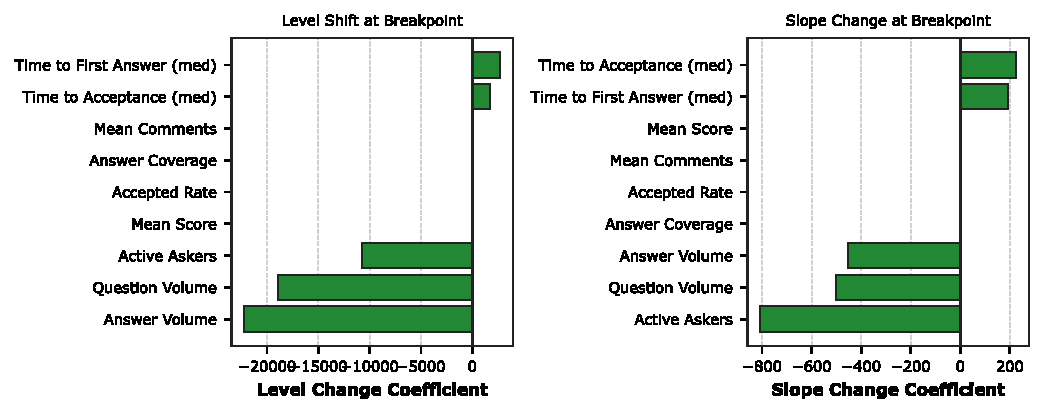
\includegraphics[width=\columnwidth]{five_its_coefficients}
  \caption{\textsc{its} level change (left)
    and slope change (right).
    Green = significant at $p < 0.05$.}
  \label{fig:its-coefs}
\end{figure}

Question volume experienced a significant
level drop ($-$\num{18960}~questions/month,
$p < 10^{-4}$) and a steepening decline
($-502$ additional questions lost per month,
$p = 0.01$).
Response times show the most dramatic
ongoing deterioration:
time-to-acceptance gains
$+226$~seconds per month
($p < 10^{-6}$),
an accelerating slowdown
that has not stabilised
by March~2026.
Mean Score dropped immediately
($-0.13$, $p = 0.004$)
but the positive slope change
($+0.021$/month, $p < 10^{-6}$)
indicates gradual recovery in
the quality of surviving questions.
Answer Coverage had no significant
level change ($p = 0.713$)
but a significant negative slope
($-0.002$/month, $p < 10^{-6}$),
indicating slow erosion
rather than an abrupt drop.

All \textsc{its} models achieve
$R^2$ values between 0.74 and 0.98;
the segmented trend model captures
the vast majority of variance.

% =====================================================================
\section{Limitations and Threats to Validity}
\label{sec:limitations}

\paragraph{Data source.}
The BigQuery snapshot ended on 2022-09-25,
which forced our pivot to the official dump.
Community-mirrored dumps
can omit posts from deleted users;
we use the official release
to minimise this gap.

\paragraph{Confounding platform events.}
Stack Overflow opened opinion-based questions
to all users in early~2026
and launched a major site redesign
between February and April~2026
(later withdrawn).
These events affect engagement
in the late period of our window.
The structural-break tests
are robust to late-period noise
because the breakpoint is fixed
at December~2022.

\paragraph{Selection bias.}
Our data covers public developer activity only.
Private AI tool usage inside companies
is invisible.
The 98.6\,\% decline in public questions
does not imply an equal decline
in developer problems,
because many of those problems
migrated to private AI interactions.

\paragraph{Interaction metrics as proxies.}
Time-to-first-answer and accepted rate
are practical signals of community behaviour,
not direct measures of developer success.

\paragraph{Classification.}
The regex-based intent classifier
operates on surface patterns.
It is transparent and reproducible
but will misclassify questions
with atypical phrasing.

% =====================================================================
\section{Conclusions}
\label{sec:conclusions}

We analysed Stack Overflow
from January~2020 through March~2026,
addressing five research questions
about the platform's transformation
in the generative AI era.

\paragraph{RQ1.}
Activity collapsed.
Monthly question volume fell 98.6\,\%;
the asker base shrank 72\,\%;
response times tripled.
Participation contraction,
rather than per-user offloading,
drives the decline.

\paragraph{RQ2.}
The surviving questions are heavier:
body prose up 32\,\%,
code content up 31\,\%,
code-block count up 18\,\%.
Every free-to-vary content dimension increased;
structurally constrained features held flat.

\paragraph{RQ3.}
The intent distribution shifted
away from \textsc{api} Usage ($-8.1$~pp)
and toward Errors ($+4.2$~pp)
and Discrepancy ($+1.9$~pp).
Machine-Authored Discrepancy grew tenfold
from 0.15\,\% to 1.50\,\%.

\paragraph{RQ4.}
All four technology domains
lost 69--76\,\% of volume.
The concept-drift hypothesis
finds only weak support;
AI/ML and Fast-Moving Web
declined marginally more
than Legacy Stable.

\paragraph{RQ5.}
Chow tests confirm significant
structural breaks
for all nine metrics at the ChatGPT release.
\textsc{its} regression reveals
both level drops and slope changes;
response-time deterioration accelerates
at $+226$~seconds per month.

The evidence supports
the AI verification tax hypothesis.
Developers have not stopped
encountering problems;
they reserve Stack Overflow
for the problems that AI cannot solve.
The platform is transitioning
from a general-purpose code reference
to a specialised venue
for error diagnosis,
architectural consensus,
and AI-code debugging.

% =====================================================================
\section{Reproducibility}
\label{sec:reproducibility}

Researcher with their own copy
of the Stack Overflow data dump
clones the repository,
sets \texttt{DATA\_DUMP} to point
at the dump location,
and runs the pipeline.
\textsc{sha}-256 checksums in
\texttt{results/tables/manifest.yaml}
allow byte-level verification.
All code, the dataset manifest,
figure-generation scripts,
and the sampling methodology
are open-source in the project repository.

\balance
\section{Statement of AI Use}
All core ideation, conceptualisation,
and research directions
are the exclusive work of the authors.
AI tools assisted with writing
and analysis.
All AI-generated suggestions were
critically reviewed;
the authors assume full responsibility
for the final content.

\bibliographystyle{ACM-Reference-Format}
\bibliography{main}

\end{document}
